\documentclass[11pt]{article}
\usepackage[margin=1in]{geometry}
\usepackage{volfit_preamble}
\graphicspath{{figures/}}

\title{\textbf{SVI and SVI-JW}\\[2pt]
\large Stochastic-volatility-inspired slices, jump-wing handles, and constrained calibration\\[2pt]
\normalsize Vol-Fitter Technical Notes, No.~02}
\author{Vol-Fitter}
\date{\today}

\begin{document}
\maketitle
% Auto-generated by gen_svi.py — do not edit.
\newcommand{\svimaxerr}{0.00}
\newcommand{\svinfev}{21}
\newcommand{\sviwingL}{0.1093}
\newcommand{\sviwingR}{0.0364}
\newcommand{\svipenalty}{1000}
\newcommand{\svileemax}{2.0}
\newcommand{\svirawtable}{\begin{tabular}{lr} \toprule Parameter & Value\\ \midrule $a$ & +0.010625\\ $b$ & +0.072887\\ $\rho$ & -0.500000\\ $m$ & +0.058310\\ $\sigma$ & +0.100995\\ \bottomrule \end{tabular}}
\newcommand{\svijwtable}{\begin{tabular}{lr} \toprule Handle & Value\\ \midrule $v$ & +0.042500\\ $\psi$ & -0.250000\\ $p$ & +0.750000\\ $c$ & +0.250000\\ $\tilde v$ & +0.034000\\ \bottomrule \end{tabular}}
\newcommand{\svianalyticms}{0.9}
\newcommand{\svifdms}{2.5}
\newcommand{\svispeedup}{2.75}
\newcommand{\svicostdiff}{3.9e-34}


\begin{abstract}
This note documents the Vol-Fitter's SVI slice model. Raw SVI parametrizes total
implied variance as a hyperbola in log-moneyness,
$w(k)=a+b\{\rho(k-m)+\sqrt{(k-m)^2+\sigma^2}\}$, with five parameters that are
geometrically opaque but analytically convenient. The \emph{jump-wing} (SVI-JW)
re-coordinatization replaces them with five quantities a trader actually quotes
--- ATM variance, ATM skew, the two wing slopes, and the minimum variance --- and
we give the exact conversion in both directions \emph{together with its exact
domain}: a jump-wing quintuple is representable at all iff $v>0$, $p,c>0$, the
quoted ATM skew lies strictly between half the wing slopes,
$-p/2<\psi<c/2$, and $\widetilde v<v$ --- with a genuine coordinate
singularity on the stratum $\psi=0$ (ATM at the vertex), where $(m,\sigma)$
is not identified by the handles. The production converter carries
\emph{no} guards, so this domain is the caller's contract, stated here
precisely. We restate the no-arbitrage conditions in JW units --- Lee's cap
becomes $\max(p,c)\sqrt{vt}\le2$ and the minimum-variance condition is
$\widetilde v\ge0$ --- show how the calibrator enforces them as two soft
penalties that vanish on any admissible slice, and explain the unconstrained
reparametrization (softplus / $\tanh$ / $\exp$) that lets a plain
Levenberg--Marquardt solver only ever propose feasible slices. As in the LQD
note, the residual Jacobian is available in closed form; a fresh run recovers
a benchmark SVI-JW smile to machine precision, reproduces its jump-wing
handles exactly, and runs \svispeedup$\times$ faster than the
finite-difference Jacobian.
\end{abstract}

\tableofcontents
\newpage

%======================================================================
\section{Why SVI, and why two parametrizations}
\label{sec:why}

SVI is the workhorse of single-slice equity-index fitting because the hyperbola
\begin{equation}
w(k)=a+b\Big\{\rho(k-m)+\sqrt{(k-m)^2+\sigma^2}\Big\}
\label{eq:rawsvi}
\end{equation}
is, in five parameters, simultaneously (i) linear in its wings ---
$w(k)\sim b(1\pm\rho)\,|k|$ --- so automatically Lee-compatible, (ii) smooth and
convex enough to be butterfly-free over a wide admissible cone, and (iii) cheap
to evaluate and differentiate. The cost is that $(a,b,\rho,m,\sigma)$ are
geometrically entangled: no single one is ``the skew'' or ``the ATM level''. The
Vol-Fitter therefore carries SVI in \emph{two} coordinate systems --- raw for the
optimizer, jump-wing for the human --- and converts losslessly between them.

\begin{invariant}
\begin{enumerate}[leftmargin=1.6em]
\item The optimizer can only propose structurally valid hyperbolas: $b\ge0$,
$|\rho|<1$, $\sigma>0$ hold by reparametrization, not by rejection.
\item The two economic no-arbitrage conditions --- non-negative minimum
variance and the Lee wing cap --- are soft hinges that are \emph{exactly zero}
on any admissible slice (byte-identical fits).
\item The raw$\leftrightarrow$JW conversion is exact on its domain
(\cref{prop:domain}); the converter itself carries no guards, so the domain is
the caller's contract.
\item SVI is a display overlay like any other: band, calendar, var-swap and
prior blocks attach identically, and each is absent-is-byte-identical.
\end{enumerate}
\end{invariant}

\begin{heuristic}
Read \eqref{eq:rawsvi} as a hyperbola: $b$ is the overall steepness (the
asymptotic opening angle), $\rho\in(-1,1)$ tilts it (left wing steeper than right
for the equity put skew $\rho<0$), $m$ shifts its vertex in $k$, $\sigma$ rounds
off the vertex (larger $\sigma$ = flatter bottom), and $a$ raises the whole curve.
The wings are straight lines of slope $b(1-\rho)$ on the left and $b(1+\rho)$ on
the right --- which is exactly what Lee's bound constrains.
\end{heuristic}

%======================================================================
\section{Raw SVI geometry}
\label{sec:raw}

The derivatives used everywhere below are
\begin{equation}
w'(k)=b\Big(\rho+\frac{k-m}{r}\Big),\qquad
w''(k)=\frac{b\,\sigma^2}{r^3},\qquad
r=\sqrt{(k-m)^2+\sigma^2}.
\label{eq:svi_deriv}
\end{equation}
Note $w''>0$ always (the slice is convex in $k$), and the wing limits are
\begin{equation}
\lim_{k\to-\infty}\frac{w(k)}{|k|}=b(1-\rho),
\qquad
\lim_{k\to+\infty}\frac{w(k)}{k}=b(1+\rho).
\label{eq:svi_wings}
\end{equation}
The vertex (minimum total variance) sits at $k^\star=m-\sigma\rho/\sqrt{1-\rho^2}$
with value $w(k^\star)=a+b\sigma\sqrt{1-\rho^2}$; this minimum is the quantity the
jump-wing parametrization calls $\widetilde v\,t$.

%======================================================================
\section{The jump-wing handles}
\label{sec:jw}

The SVI-JW parametrization $(v,\psi,p,c,\widetilde v)$ at expiry $t$ is defined by
ATM and wing functionals of the slice:
\begin{equation}
\begin{aligned}
v&=\frac{w(0)}{t} && \text{ATM variance,}\\
\psi&=\frac{b}{2\sqrt{w_0}}\Big(\rho-\frac{m}{\sqrt{m^2+\sigma^2}}\Big) && \text{ATM skew,}\\
p&=\frac{b(1-\rho)}{\sqrt{w_0}},\quad c=\frac{b(1+\rho)}{\sqrt{w_0}} && \text{put/call wing slopes,}\\
\widetilde v&=\frac{a+b\sigma\sqrt{1-\rho^2}}{t} && \text{minimum variance,}
\end{aligned}
\label{eq:jw_def}
\end{equation}
with $w_0=w(0)=vt$. \Cref{fig:jw} annotates the five handles on a fitted smile.

\begin{figure}[H]
\centering
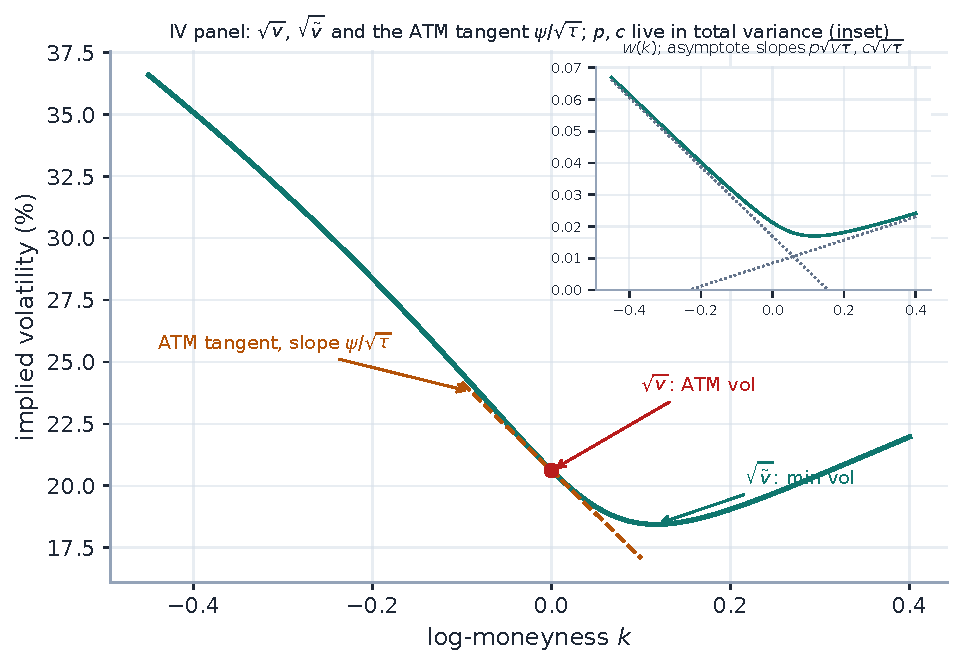
\includegraphics[width=0.78\textwidth]{fig_svi_jw.pdf}
\caption{The five SVI-JW handles read off a fitted slice: ATM variance $v$, ATM
skew $\psi$, put/call wing slopes $p,c$, and minimum variance $\widetilde v$.}
\label{fig:jw}
\end{figure}

\subsection{The conversion, both ways}

Going \emph{from} jump-wing \emph{to} raw is what the app stores when a desk
quotes handles. Set $w_0=vt$, $\sqrt{w_0}=\sqrt{vt}$, and
\begin{equation}
b=\frac{\sqrt{w_0}}{2}(p+c),\qquad \rho=\frac{c-p}{c+p},\qquad
\chi:=\frac{m}{\sqrt{m^2+\sigma^2}}=\rho-\frac{4\psi}{p+c}.
\label{eq:jw_to_raw_1}
\end{equation}
From $\chi$ one recovers $m=\chi\sigma/\sqrt{1-\chi^2}$ and
$\sqrt{m^2+\sigma^2}=\sigma/\sqrt{1-\chi^2}$; subtracting the minimum-variance
identity from the ATM identity gives the closed form
\begin{equation}
\sigma=\frac{w_0-\widetilde v\,t}{b\big((1-\rho\chi)/\sqrt{1-\chi^2}-\sqrt{1-\rho^2}\big)},
\qquad a=\widetilde v\,t-b\sigma\sqrt{1-\rho^2}.
\label{eq:jw_to_raw_2}
\end{equation}
The reverse map \emph{from} raw \emph{to} jump-wing is just the definitions
\eqref{eq:jw_def} evaluated on the fitted raw slice. (Two precisions about
what production actually runs: the backend ships only the forward converter
\texttt{jw\_to\_raw} --- the reverse map lives in the figure generator and in
these equations --- and the \emph{live} smile panel displays the three
model-agnostic numeric handles ATM vol/skew/curvature by finite differences,
not the five closed-form JW handles.) \Cref{sec:example} verifies the
round-trip numerically to machine precision. The forward conversion
\eqref{eq:jw_to_raw_1}--\eqref{eq:jw_to_raw_2} is direct:

\begin{lstlisting}[caption={SVI-JW handles $\to$ raw SVI (distilled from
\texttt{models/svi\_jw/svi.py}; agrees with it to $10^{-12}$).},label={lst:jw2raw}]
def jw_to_raw(t, v, psi, p, c, vt):          # v, psi, p, c, vtilde  ->  a, b, rho, m, sigma
    w0 = v*t; sq = np.sqrt(w0)
    b = 0.5*sq*(p + c)
    rho = (c - p)/(c + p)
    chi = rho - 4*psi/(p + c)                # chi = m / sqrt(m^2 + sigma^2)
    r1x, r1r = np.sqrt(1 - chi*chi), np.sqrt(1 - rho*rho)
    sigma = (w0 - vt*t) / (b*((1 - rho*chi)/r1x - r1r))
    m = chi*sigma/r1x
    a = vt*t - b*sigma*r1r
    return a, b, rho, m, sigma
\end{lstlisting}

\subsection{The conversion domain, exactly}
\label{sec:domain}

Not every quintuple $(v,\psi,p,c,\widetilde v)$ is a smile. The formulas above
divide by $p+c$, by $\sqrt{1-\chi^2}$ and by the bracket in
\eqref{eq:jw_to_raw_2}, and the production converter carries \emph{no} guards
--- so the exact domain is worth stating and proving.

\begin{proposition}[Conversion domain]
\label{prop:domain}
Fix $t>0$. The map \eqref{eq:jw_to_raw_1}--\eqref{eq:jw_to_raw_2} produces a
valid raw slice ($b>0$, $|\rho|<1$, $\sigma>0$, $m$ finite) if and only if
\[
v>0,\qquad p>0,\ c>0,\qquad -\frac{p}{2}<\psi<\frac{c}{2},\qquad
\psi\neq0,\qquad \widetilde v<v .
\]
In words: the wings must be genuinely upward, the quoted ATM skew must lie
strictly between \emph{half the wing slopes}, and the ATM variance must sit
strictly above the minimum.
\end{proposition}

\begin{proof}
$p,c>0$ gives $b=\tfrac{\sqrt{w_0}}{2}(p+c)>0$ and
$\rho=(c-p)/(c+p)\in(-1,1)$. For $\chi=\rho-4\psi/(p+c)$, using
$(\rho-1)(p+c)=-2p$ and $(\rho+1)(p+c)=2c$,
\[
|\chi|<1
\iff \frac{(\rho-1)(p+c)}{4}<\psi<\frac{(\rho+1)(p+c)}{4}
\iff -\frac p2<\psi<\frac c2 ,
\]
which keeps $m=\chi\sigma/\sqrt{1-\chi^2}$ finite. For $\sigma$: by
Cauchy--Schwarz applied to the unit vectors $(\rho,\sqrt{1-\rho^2})$ and
$(\chi,\sqrt{1-\chi^2})$,
\[
\rho\chi+\sqrt{1-\rho^2}\sqrt{1-\chi^2}\le1,
\quad\text{i.e.}\quad
\frac{1-\rho\chi}{\sqrt{1-\chi^2}}\ \ge\ \sqrt{1-\rho^2},
\]
with equality iff $\chi=\rho$, i.e.\ iff $\psi=0$. So the bracket in
\eqref{eq:jw_to_raw_2} is strictly positive exactly when $\psi\neq0$, and
$\sigma>0$ then requires the numerator $w_0-\widetilde vt>0$, i.e.\
$\widetilde v<v$. Conversely each failure breaks a requirement: $p+c\le0$
kills $b$ or $\rho$; $\psi$ outside the band sends $|\chi|\ge1$ ($m$
infinite); $\psi=0$ zeroes the bracket; $\widetilde v\ge v$ makes
$\sigma\le0$.
\end{proof}

\begin{remark}[The $\psi=0$ stratum is a genuine coordinate singularity]
\label{rem:psi0}
On a true SVI slice, $\psi=0$ means $\chi=\rho$, which happens exactly when
the ATM point \emph{is} the vertex --- and then $\widetilde v=v$
automatically. On that stratum the five handles do not identify the slice:
for any $\sigma>0$, the raw slice with $m=\rho\sigma/\sqrt{1-\rho^2}$ and
$a=\widetilde vt-b\sigma\sqrt{1-\rho^2}$ reproduces the \emph{same}
$(v,0,p,c,v)$ --- the handles omit ATM curvature, and this is where it shows.
The jump-wing chart is a fine trader coordinate system \emph{away} from the
symmetric-vertex stratum, and ill-conditioned near it: as $\psi\to0$, the
conversion computes $\sigma$ as a ratio of two vanishing quantities, with
catastrophic cancellation before the limit.
\end{remark}

\begin{caution}
The production \texttt{jw\_to\_raw} implements the formulas verbatim with
\emph{zero} domain checks: $p+c=0$ or $|\chi|\ge1$ divides by zero silently,
and a near-zero $\psi$ silently amplifies rounding. This is deliberate ---
the converter's only callers feed it benchmark or desk handles comfortably
inside \cref{prop:domain} --- but it makes the domain a \emph{contract}, not
a runtime guarantee. Anyone wiring JW handles to user input must validate
against \cref{prop:domain} first; the note, not the code, is the fence.
\end{caution}

%======================================================================
\section{Static no-arbitrage}
\label{sec:noarb}

\subsection{Butterfly: Durrleman's function}

A slice is free of butterfly arbitrage iff the risk-neutral density it implies is
non-negative, which Durrleman's condition expresses directly on total variance:
\begin{equation}
g(k)=\Big(1-\frac{k\,w'(k)}{2w(k)}\Big)^2-\frac{w'(k)^2}{4}\Big(\frac{1}{w(k)}+\frac14\Big)+\frac{w''(k)}{2}\ \ge\ 0
\quad\forall k.
\label{eq:durrleman}
\end{equation}
For raw SVI, $g$ is a smooth function of \eqref{eq:rawsvi}--\eqref{eq:svi_deriv}
with no closed-form sign. In production it is evaluated as the closed-form
$(w,w',w'')$ triple by the backtest's analytic arbitrage metric (Note~09) and
by the note's own figures; the fit itself does not carry a $g$ hinge --- the
Gatheral--Jacquier parameter-space conditions bound the wing steepness
$b(1+|\rho|)$ and the minimum total variance, and the calibrator enforces the
two that bite in practice.

How $g$ is \emph{measured} matters as much as what it says. An earlier
backtest metric evaluated $g$ by finite differences of reconstructed option
prices, and its numerical noise flagged $28.3\%$ of provably-clean LQD slices
as arbitrageable; recomputed analytically from each model's own
$(w,w',w'')$, the LQD rate reads $0.0\%$, and SVI's flagged rate fell from
$20.8\%$ to $9.2\%$ --- the survivors being genuine: the two soft hinges below
fence the conditions that bite, they do not certify $g\ge0$ pointwise. The
production rule that came out of that audit is that the diagnostic is always
computed on model derivatives, never by differencing prices (Note~09 has the
cross-model treatment).

\begin{proposition}[The enforced conditions, in JW units]
\label{prop:jwnoarb}
Under the conversion of \cref{sec:jw}, the two coded penalties read directly
on the trader handles: the minimum-variance condition
$a+b\sigma\sqrt{1-\rho^2}\ge0$ is exactly $\widetilde v\ge0$, and Lee's cap
$b(1+|\rho|)\le\beta_{\max}$ is exactly
\[
\max(p,c)\,\sqrt{vt}\ \le\ \beta_{\max}\ (=2).
\]
\end{proposition}

\begin{proof}
The first is the definition of $\widetilde v$ in \eqref{eq:jw_def} times
$t>0$. For the second, $b(1\mp\rho)=p\sqrt{w_0}$ and $c\sqrt{w_0}$
respectively by \eqref{eq:jw_def}, so
$b(1+|\rho|)=\max\big(b(1-\rho),b(1+\rho)\big)=\max(p,c)\sqrt{w_0}$ with
$w_0=vt$.
\end{proof}

So a desk can sanity-check a handle quote before any conversion: wings
non-negative at the vertex ($\widetilde v\ge0$), skew inside
$(-p/2,\,c/2)$ (\cref{prop:domain}), and $\max(p,c)\sqrt{vt}\le2$ (Lee).

\subsection{The two soft penalties}

The optimizer adds, to the data residual, two penalties that are \emph{exactly
zero} on an admissible slice and grow linearly past the boundary:
\begin{equation}
\rho_{\text{pen}}(\theta)=W\!\begin{pmatrix}
\max\big(-(a+b\sigma\sqrt{1-\rho^2}),\,0\big)\\[2pt]
\max\big(b(1+|\rho|)-\beta_{\max},\,0\big)
\end{pmatrix},
\label{eq:svi_penalties}
\end{equation}
with weight $W=\svipenalty$ and Lee cap $\beta_{\max}=\svileemax$. The first
keeps the \emph{minimum total variance} non-negative (no negative density mass at
the vertex); the second enforces Lee's bound that the asymptotic total-variance
slope cannot exceed $2$. Because both vanish on a clean fit, an admissible smile
(such as the benchmark of \cref{sec:example}) is byte-identical with or without
them --- they are a feasibility fence, not a regularizer.

\begin{caution}
The penalty weight $W=\svipenalty$ is in $\mathrm{vol}^2$ units, deliberately
large enough to dominate a violated constraint yet invisible on an admissible
slice. It is \emph{not} a tuning dial for fit quality: raising it cannot improve
a feasible fit, and lowering it only lets the optimizer wander into the
arbitrageable cone. Note~09 develops the Lee bound across all the models; here it
is one of these two hinges.
\end{caution}

%======================================================================
\section{Calibration}
\label{sec:calib}

\subsection{Unconstrained reparametrization}

Rather than run a bound-constrained optimizer, the Vol-Fitter reparametrizes so
that \emph{every} point of $\R^5$ maps to an admissible raw slice:
\begin{equation}
a\ \text{free},\quad
b=\operatorname{softplus}(\theta_b)\ge 0,\quad
\rho=\tanh(\theta_\rho)\in(-1,1),\quad
m\ \text{free},\quad
\sigma=e^{\theta_\sigma}>0.
\label{eq:reparam}
\end{equation}
This guarantees $b\ge0$, $|\rho|<1$, $\sigma>0$ for free, so the unconstrained
Levenberg--Marquardt solver never wastes effort on the box and never proposes a
nonsensical hyperbola; only the two \emph{economic} constraints
\eqref{eq:svi_penalties} remain, and they are soft.

\subsection{Objective, weights and the data-driven start}

The data term is a plain implied-volatility residual,
$r_i=\sqrt{\omega_i}\,(\sigma^{\text{SVI}}(k_i)-\sigma_i)$, optionally
vega-weighted (pass $\omega_i=\text{vega}_i^2$). The initializer is geometric and
reads the smile directly: the argmin of $w$ seeds $(a,m)$, and the two finite
wing slopes seed $(b,\rho)$ via \eqref{eq:svi_wings}, then the reparametrization
\eqref{eq:reparam} is inverted to get $\theta_0$. On a liquid smile a single LM
pass converges from this start.

\subsection{The analytic Jacobian and the optional blocks}

The residual stack --- data (mid or band), the two penalties, and an optional
calendar hinge --- has a closed-form Jacobian propagated through the
reparametrization \eqref{eq:reparam} by the chain rule; the calibrator uses it
whenever no var-swap or prior block is present (those are not yet differentiated
and fall back to finite differences, exactly as in LQD). The optional blocks
mirror the rest of the series:
\begin{itemize}[leftmargin=1.4em]
\item \textbf{Band fit} (Note~07): the mid residual becomes a vol-space band
hinge with a small mid anchor.
\item \textbf{Calendar hinge} (Note~10): the \emph{model-agnostic} constraint
$\sqrt{W_{\text{cal}}}\,\max(\text{floor}-w(k),0)$ keeps this slice's total
variance at or above the nearer expiry's --- the same machinery LQD expresses via
its quantile $A(z)$, here written directly on $w(k)$.
\item \textbf{Var-swap target} (Note~08) and \textbf{prior persistence}
(Note~13): added as in LQD, so the SVI \emph{display overlay} receives the same
prior treatment as the primary model --- closing a long-standing asymmetry in
which SVI overlays got no prior at all.
\end{itemize}

\begin{perfbox}
The solver is Levenberg--Marquardt (\texttt{method="lm"}), not trust-region
reflective. On noisy real chains LM crosses the penalty kinks in far fewer
iterations than \texttt{trf} at matched tolerance, so it is the faster
same-accuracy choice; the analytic Jacobian is then a drop-in that swaps scipy's
$1+P$ finite-difference evaluations for one closed-form call. It shipped after
the offline backtest (project \texttt{backtest/}) identified those
finite-difference evaluations as SVI's dominant fit cost: on real spike-regime
nodes the swap measured $26.3\to10.2$\,ms per fit ($\approx2.6\times$) at
unchanged convergence --- same optimizer, same tolerances, identical solution.
\Cref{sec:example} measures \svispeedup$\times$ on this note's benchmark with
the optimum unchanged to $\svicostdiff$ in cost. See \cref{app:perf}.
\end{perfbox}

%======================================================================
\section{Worked example: round-trip recovery}
\label{sec:example}

The cleanest test of an SVI-JW implementation is a round trip. Take the SPX-like
benchmark raw slice $(a,b,\rho,m,\sigma)=(0.010625,\,0.07289,\,-0.5,\,0.05831,\,
0.10100)$ at $t=0.5$ --- the image under \eqref{eq:jw_to_raw_1}--\eqref{eq:jw_to_raw_2}
of the jump-wing handles $(v,\psi,p,c,\widetilde v)=(0.0425,-0.25,0.75,0.25,0.034)$.
Generate quotes from it, refit raw SVI from the geometric start, and read the
handles back.

The fit recovers the raw parameters (\cref{tab:svi_raw}) with a maximum
implied-volatility error of \svimaxerr\ volatility basis points in \svinfev\
residual evaluations, the wing slopes come out $b(1-\rho)=\sviwingL$ (put) and
$b(1+\rho)=\sviwingR$ (call), and --- the point of the exercise --- the recovered
jump-wing handles (\cref{tab:svi_jw}) reproduce the original
$(0.0425,-0.25,0.75,0.25,0.034)$ to display precision. The conversion
\eqref{eq:jw_def}--\eqref{eq:jw_to_raw_2} is therefore exact, not approximate.
\Cref{fig:fit} shows the fit and \cref{fig:g} the Durrleman function staying
non-negative across the strike range.

\begin{table}[H]
\centering
\begin{minipage}{0.46\textwidth}\centering
\caption{Recovered raw SVI.}\label{tab:svi_raw}
\svirawtable
\end{minipage}\hfill
\begin{minipage}{0.46\textwidth}\centering
\caption{Recovered SVI-JW handles.}\label{tab:svi_jw}
\svijwtable
\end{minipage}
\end{table}

\begin{figure}[H]
\centering
\begin{minipage}{0.49\textwidth}\centering
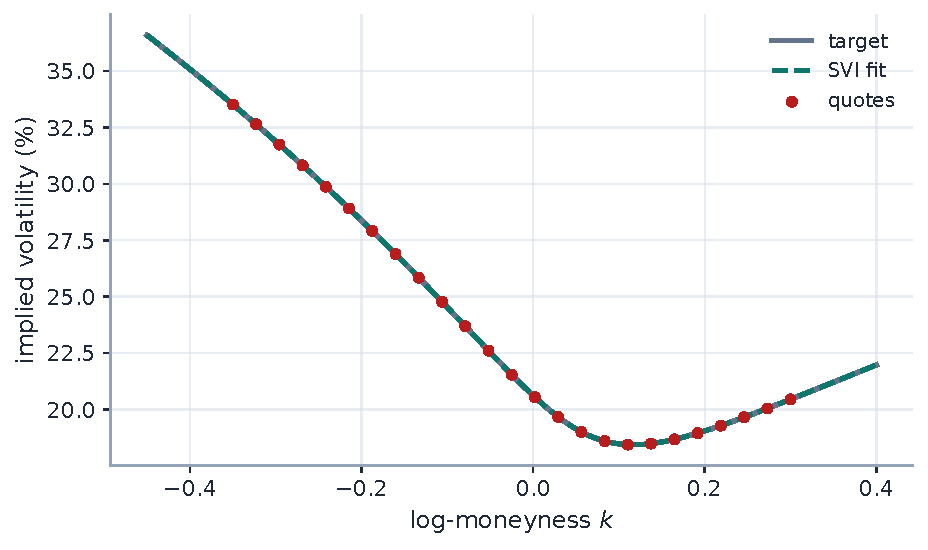
\includegraphics[width=\textwidth]{fig_svi_fit.pdf}\\[1pt]
{\footnotesize (a) target, fit, quotes}
\end{minipage}\hfill
\begin{minipage}{0.49\textwidth}\centering
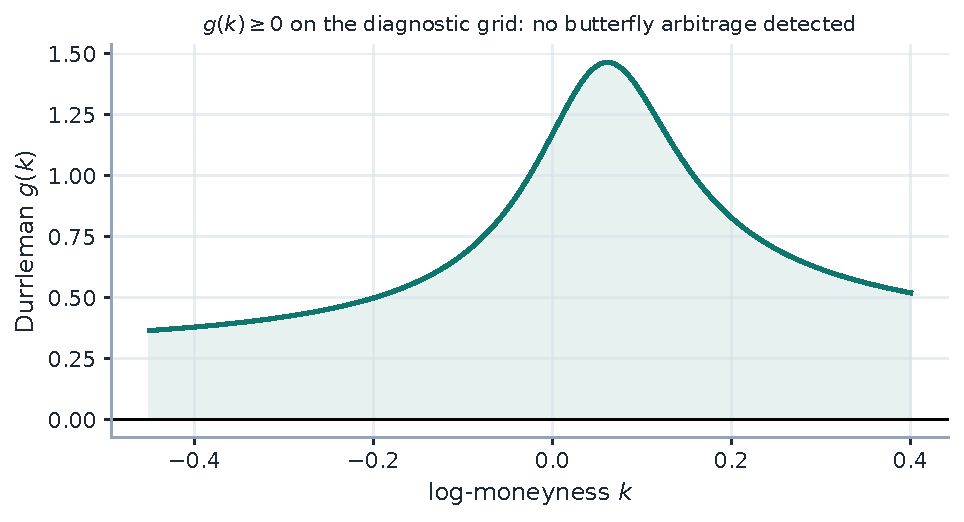
\includegraphics[width=\textwidth]{fig_svi_g.pdf}\\[1pt]
{\footnotesize (b) Durrleman $g(k)\geq0$}
\end{minipage}
\caption{Left: the benchmark smile and its SVI fit (max error \svimaxerr\ vol
bps). Right: the butterfly diagnostic $g(k)$, positive throughout.}
\label{fig:fit}
\end{figure}
\begin{figure}[H]\centering\phantomsection\label{fig:g}\end{figure}

\begin{heuristic}
A round-trip error of \svimaxerr\ vol bps is expected because the target \emph{is}
an SVI slice --- the exercise validates the optimizer and the conversion, not the
expressiveness of SVI. On genuine market chains SVI typically fits liquid index
smiles to a few vol bps but is stiffer than LQD or Local-Vol on event or
double-hump shapes (a single hyperbola has one vertex), which is precisely why
the app offers the other models.
\end{heuristic}

%======================================================================
\section{What is original here, and limitations}
\label{sec:original}

SVI and the jump-wing handles are due to Gatheral; the arbitrage-free analysis is
Gatheral--Jacquier and Durrleman. The implementation choices worth noting are the
\emph{feasibility-by-reparametrization} \eqref{eq:reparam} (the solver cannot
leave the admissible cone except through the two soft economic constraints), the
\emph{closed-form raw$\leftrightarrow$JW round trip} used live for trader handles,
and the \emph{analytic LM Jacobian} that makes SVI the speed peer of the other
models. As a slice model SVI is intrinsically unimodal: it cannot represent a
bimodal event density (Note~01's double-hat) or a WW-shaped smile (Note~03), and
its single global hyperbola can over-smooth a sharp short-dated skew. It is
butterfly-free only over its admissible cone --- enforced softly here --- and
carries no calendar coupling on its own; that is supplied by the model-agnostic
hinge of Note~10.

%======================================================================
\section{Traceability}
\label{sec:traceability}

\begingroup
\small
\setlength{\tabcolsep}{3pt}
\begin{longtable}{@{}p{0.30\textwidth}p{0.13\textwidth}p{0.25\textwidth}p{0.28\textwidth}@{}}
\caption{Claims in this note and the code/tests that lock them.}\\
\toprule Claim & Object & Code anchor & Test anchor\\ \midrule
\endfirsthead
\toprule Claim & Object & Code anchor & Test anchor\\ \midrule
\endhead
JW$\to$raw conversion exact on the benchmark &
\cref{sec:jw} &
\nolinkurl{models/svi_jw/svi.py::jw_to_raw} &
\nolinkurl{test_lqd_pricing.py::test_jw_conversion_matches_note}\\
Round trip: parameters and curve recovered &
\cref{sec:example} &
\nolinkurl{models/svi_jw/calibrate.py} &
\nolinkurl{test_svi_calibrate.py::test_recovers_benchmark_parameters}, \nolinkurl{::test_curve_reproduced_to_machine_precision}\\
Lee cap enforced &
\cref{prop:jwnoarb} &
\nolinkurl{models/svi_jw/calibrate.py::_penalties} &
\nolinkurl{test_svi_calibrate.py::test_respects_lee_wing_bound}\\
Minimum variance non-negative &
\cref{prop:jwnoarb} &
\nolinkurl{models/svi_jw/calibrate.py::_penalties} &
\nolinkurl{test_svi_calibrate.py::test_min_variance_non_negative}\\
Analytic Jacobian $=$ FD, penalties active or not &
\cref{sec:calib} &
\nolinkurl{models/svi_jw/jacobian.py} &
\nolinkurl{test_svi_jacobian.py::test_mid_fit_admissible}, \nolinkurl{::test_lee_penalty_active}, \nolinkurl{::test_min_variance_penalty_active}\\
Calendar hinge rows correct &
\cref{sec:calib} &
\nolinkurl{models/svi_jw/calibrate.py} &
\nolinkurl{test_svi_jacobian.py::test_calendar_floor_active}, \nolinkurl{test_overlay_calendar.py::test_svi_no_floor_is_byte_identical}\\
Vega-weighted fit supported &
\cref{sec:calib} &
\nolinkurl{models/svi_jw/calibrate.py::_vega_weights} &
\nolinkurl{test_svi_calibrate.py::test_recovers_under_vega_weights}\\
Prior blocks reach the SVI overlay &
\cref{sec:calib} &
\nolinkurl{models/svi_jw/calibrate.py} &
\nolinkurl{test_prior_parametric.py::test_operator_prior_pulls_all_models_toward_prior_skew}\\
\bottomrule
\end{longtable}
\endgroup

\noindent The conversion-domain conditions of \cref{prop:domain} are a
\emph{documented contract}, not code: the converter has no guards and no
domain test. That is a known, deliberate gap --- flagged here so it cannot be
mistaken for an enforced invariant.

\appendix
%======================================================================
\section{Hyperparameter atlas}
\label{app:atlas}

\begin{longtable}{p{0.24\textwidth}p{0.13\textwidth}p{0.55\textwidth}}
\caption{SVI hyperparameters.}\label{tab:atlas}\\
\toprule Knob & Default & Role\\ \midrule
\endfirsthead
\toprule Knob & Default & Role\\ \midrule
\endhead
\multicolumn{3}{l}{\emph{Surfaced (FitSettings)}}\\ \midrule
\texttt{sviPenaltyWeight} $W$ & \svipenalty & Weight of the two soft
no-arbitrage penalties \eqref{eq:svi_penalties}; $\mathrm{vol}^2$ units.\\
\texttt{leeSlopeMax} $\beta_{\max}$ & \svileemax & Lee wing-slope cap; the
asymptotic total-variance slope $b(1+|\rho|)$ may not exceed it.\\
\texttt{midAnchorWeight} & $0.05$ & Mid anchor weight in the band-fit objective
(Note~07).\\
\texttt{weightScheme} & \texttt{equal} & Per-quote weights (Note~07); pass
$\text{vega}^2$ for a vega-weighted fit.\\
\texttt{calendarWeight} & $10^{6}$ & Calendar hinge penalty (Note~10; lives
in \texttt{OptionsSettings}, not \texttt{FitSettings}).\\
\midrule
\multicolumn{3}{l}{\emph{Internal (reparametrization / solver)}}\\ \midrule
$b=\operatorname{softplus}(\theta_b)$ & --- & Enforces $b\ge0$.\\
$\rho=\tanh(\theta_\rho)$ & --- & Enforces $|\rho|<1$.\\
$\sigma=e^{\theta_\sigma}$ & --- & Enforces $\sigma>0$.\\
LM tolerances & $10^{-15}$ & \texttt{xtol/ftol/gtol}; LM converges in few
iterations so tight tolerances are cheap.\\
floor $10^{-12}$ & --- & Total-variance floor inside $\sqrt{w/t}$ to avoid
$\sqrt{\text{neg}}$ on infeasible trial slices.\\
\bottomrule
\end{longtable}

%======================================================================
\section{Performance notes}
\label{app:perf}

\begin{enumerate}[leftmargin=1.6em]
\item \textbf{Levenberg--Marquardt over trust-region.} On real noisy chains LM
crosses the penalty kinks in fewer iterations than \texttt{trf} at matched
tolerance; \texttt{trf} at $10^{-10}$ was measured \emph{slower} on real nodes.
\item \textbf{Analytic Jacobian.} Closed-form Jacobian of the residual stack
(data $+$ penalties $+$ calendar) through the reparametrization; a fresh run
measured \svianalyticms\,ms vs \svifdms\,ms for the finite-difference path
(\svispeedup$\times$) with the optimum unchanged to $\svicostdiff$ in cost.
On production-sized real chains (spike-regime backtest nodes) the same swap
measured $26.3\to10.2$\,ms per fit ($\approx2.6\times$) --- the backtest
finding that motivated shipping it. Gated to the var-swap/prior-free
configuration.
\item \textbf{Feasibility by construction.} The reparametrization removes the
box-constraint handling entirely, so each LM step is a plain linear solve.
\item \textbf{Geometric warm start.} Reading $(a,m)$ from the vertex and
$(b,\rho)$ from the wing slopes lands $\theta_0$ close enough that liquid smiles
converge in a single pass.
\end{enumerate}

%======================================================================
\section{Reference implementation: the reverse map}
\label{app:ref}

The raw slice evaluates in one line, $w(k)=a+b(\rho(k-m)+\sqrt{(k-m)^2+\sigma^2})$;
the reverse conversion \eqref{eq:jw_def} reads the five jump-wing handles off it.
Composing with \cref{lst:jw2raw} recovers the original handles to $10^{-10}$ --- the
round trip is exact, not approximate.

\begin{lstlisting}[caption={Raw SVI evaluation (the
\texttt{RawSVI.total\_variance} method) and the reverse map raw $\to$ SVI-JW
--- the equations \eqref{eq:jw_def}; the backend ships only the forward
converter, and this reverse listing is the one the figure generator runs.}]
def w_svi(k, a, b, rho, m, sigma):           # the hyperbola w(k)
    km = k - m
    return a + b*(rho*km + np.sqrt(km*km + sigma**2))

def raw_to_jw(t, a, b, rho, m, sigma):       # a, b, rho, m, sigma  ->  v, psi, p, c, vtilde
    w0 = w_svi(0.0, a, b, rho, m, sigma); sq = np.sqrt(w0)
    v = w0/t                                 # ATM variance
    psi = b/(2*sq)*(rho - m/np.sqrt(m*m + sigma**2))          # ATM skew
    p, c = b*(1 - rho)/sq, b*(1 + rho)/sq    # put / call wing slopes
    vt = (a + b*sigma*np.sqrt(1 - rho*rho))/t                 # minimum variance
    return v, psi, p, c, vt
\end{lstlisting}

\begin{thebibliography}{9}
\bibitem{Gatheral2004} J.~Gatheral. A parsimonious arbitrage-free implied
volatility parameterization. Presentation, Global Derivatives, 2004.
\bibitem{GatheralJacquier2014} J.~Gatheral and A.~Jacquier. Arbitrage-free SVI
volatility surfaces. \emph{Quantitative Finance}, 14(1):59--71, 2014.
\bibitem{Lee2004} R.~W.~Lee. The moment formula for implied volatility at extreme
strikes. \emph{Mathematical Finance}, 14(3):469--480, 2004.
\bibitem{Durrleman2010} V.~Durrleman. From implied to spot volatilities.
\emph{Finance and Stochastics}, 14(2):157--177, 2010.
\end{thebibliography}

\end{document}
